
%(BEGIN_QUESTION)
% Copyright 2010, Tony R. Kuphaldt, released under the Creative Commons Attribution License (v 1.0)
% This means you may do almost anything with this work of mine, so long as you give me proper credit

When sulfur-containing fuels are burned, one of the reaction products is sulfur dioxide (SO$_{2}$), which is an atmospheric pollutant.  Fortunately, SO$_{2}$ is relatively easy to ``scrub'' out of hot flue gases by spraying a liquid solution down on the rising gases and then chemically treating (regenerating) that scrubbing solution:

$$\includegraphics[width=15.5cm]{i01867x01.eps}$$

After years of successful operation, the level control loop begins to exhibit problems.  The liquid level inside the scrubbing tower mysteriously drops far below setpoint, as indicated by the level gauge (LG) on the side of the scrubber.  The operators have tried to rectify this problem by increasing the setpoint adjustment on the level controller (LC), to no avail.

Identify the likelihood of each specified fault for this level control system.  Consider each fault one at a time (i.e. no coincidental faults), determining whether or not each fault could independently account for {\it all} measurements and symptoms.

% No blank lines allowed between lines of an \halign structure!
% I use comments (%) instead, so that TeX doesn't choke.

$$\vbox{\offinterlineskip
\halign{\strut
\vrule \quad\hfil # \ \hfil & 
\vrule \quad\hfil # \ \hfil & 
\vrule \quad\hfil # \ \hfil \vrule \cr
\noalign{\hrule}
%
% First row
{\bf Fault} & {\bf Possible} & {\bf Impossible} \cr
%
\noalign{\hrule}
%
% Another row
Air supply to LT shut off &  &  \cr
%
\noalign{\hrule}
%
% Another row
Air supply to LC shut off &  &  \cr
%
\noalign{\hrule}
%
% Another row
Pump shut off &  &  \cr
%
\noalign{\hrule}
%
% Another row
Broken air line between LT and LC &  &  \cr
%
\noalign{\hrule}
%
% Another row
Broken air line between LC and LV &  &  \cr
%
\noalign{\hrule}
%
% Another row
Plugged nozzle inside LC &  &  \cr
%
\noalign{\hrule}
%
% Another row
Plugged orifice inside LC &  &  \cr
%
\noalign{\hrule}
%
% Another row
Leak in bottom of scrubber &  &  \cr
%
\noalign{\hrule}
} % End of \halign 
}$$ % End of \vbox

Finally, identify the {\it next} diagnostic test or measurement you would make on this system.  Explain how the result(s) of this next test or measurement help further identify the location and/or nature of the fault.

\underbar{file i01867}
%(END_QUESTION)





%(BEGIN_ANSWER)

% No blank lines allowed between lines of an \halign structure!
% I use comments (%) instead, so that TeX doesn't choke.

$$\vbox{\offinterlineskip
\halign{\strut
\vrule \quad\hfil # \ \hfil & 
\vrule \quad\hfil # \ \hfil & 
\vrule \quad\hfil # \ \hfil \vrule \cr
\noalign{\hrule}
%
% First row
{\bf Fault} & {\bf Possible} & {\bf Impossible} \cr
%
\noalign{\hrule}
%
% Another row
Air supply to LT shut off &  & $\surd$ \cr
%
\noalign{\hrule}
%
% Another row
Air supply to LC shut off &  & $\surd$ \cr
%
\noalign{\hrule}
%
% Another row
Pump shut off &  & $\surd$ \cr
%
\noalign{\hrule}
%
% Another row
Broken air line between LT and LC &  & $\surd$ \cr
%
\noalign{\hrule}
%
% Another row
Broken air line between LC and LV &  & $\surd$ \cr
%
\noalign{\hrule}
%
% Another row
Plugged nozzle inside LC & $\surd$ &  \cr
%
\noalign{\hrule}
%
% Another row
Plugged orifice inside LC &  & $\surd$ \cr
%
\noalign{\hrule}
%
% Another row
Leak in bottom of scrubber & $\surd$ &  \cr
%
\noalign{\hrule}
} % End of \halign 
}$$ % End of \vbox

%(END_ANSWER)





%(BEGIN_NOTES)

A good ``next step'' is to check the stem position of the LV, to see if the valve is open or not.  If the level is far below setpoint, the level controller should be trying to shut off the valve.  If the valve is not shutting, it could be a valve problem or a controller problem.  If the valve is shutting, it could be a leaking valve or a leaking scrubber.

\vskip 20pt \vbox{\hrule \hbox{\strut \vrule{} {\bf Virtual Troubleshooting} \vrule} \hrule}

This question is a good candidate for a ``Virtual Troubleshooting'' exercise.  Presenting the diagram to students, you first imagine in your own mind a particular fault in the system.  Then, you present one or more symptoms of that fault (something noticeable by an operator or other user of the system).  Students then propose various diagnostic tests to perform on this system to identify the nature and location of the fault, as though they were technicians trying to troubleshoot the problem.  Your job is to tell them what the result(s) would be for each of the proposed diagnostic tests, documenting those results where all the students can see.

During and after the exercise, it is good to ask students follow-up questions such as:

\begin{itemize}
\item{} What does the result of the last diagnostic test tell you about the fault?
\item{} Suppose the results of the last diagnostic test were different.  What then would that result tell you about the fault?
\item{} Is the last diagnostic test the best one we could do?
\item{} What would be the ideal order of tests, to diagnose the problem in as few steps as possible?
\end{itemize}

\vfil \eject

\noindent
{\bf Summary Quiz:}

Suppose the pneumatic signal line between the controller and the valve suddenly breaks open (i.e. suffers a major leak).  Determine the resulting effect on the process:

$$\includegraphics[width=15.5cm]{i01867x01.eps}$$

\begin{itemize}
\item{} The actual liquid level inside the scrubber will increase
\vskip 5pt
\item{} The level transmitter will show more level than there actually is 
\vskip 5pt
\item{} The level transmitter will show less level than there actually is
\vskip 5pt
\item{} The actual liquid level inside the scrubber will decrease
\vskip 5pt
\item{} The actual liquid level inside the scrubber will remain at setpoint
\vskip 5pt
\item{} The pump will become dead-headed (no flow through it)
\end{itemize}

%INDEX% Basics, control loop troubleshooting: determining effect of process valve problem
%INDEX% Process: flue gas "wet" scrubber 
%INDEX% Troubleshooting review: electric circuits

%(END_NOTES)


